%%%%%%%%%%%%%%%%%%%%%%%%%%%%%%%%%%%%%%%%%%%%%%%%%%%%%%%%%%%%%%%%%%%%%%%%
%                                                                      %
%     File: Thesis_Applications.tex                                    %
%     Tex Master: Thesis.tex                                           %
%                                                                      %
%     Author: João D. Lopes                                            %
%     Last modified :  18 April 2017                                   %
%                                                                      %
%%%%%%%%%%%%%%%%%%%%%%%%%%%%%%%%%%%%%%%%%%%%%%%%%%%%%%%%%%%%%%%%%%%%%%%%

\chapter{Applications}
\label{chapter:applications}

The Versat architecture is suitable to be used in ultra low energy
applications such as those found in Wireless Sensor Networks (WSNs),
where using a GPU or FPGA accelerator is out of the question. A
dedicated hardware accelerator may also be used but its lack of
programmability can become a serious liability in the long run. In
this chapter, two algorithms that can be used in such applications are
presented: the Fast Fourier Transform and the K-Means Clustering
algorithms. Their implementation on Versat demonstrates the
versatility of the architecture.

% ----------------------------------------------------------------------
\section{Fast Fourier Transform }
\label{section:FFT}

The Fast Fourier Transform (FFT) is an algorithm for efficiently
computing the Discrete Fourier Transform (DFT) of a digitized
signal. It is used in many signal processing applications such as
filters, audio and video pre and post processing, as well as encoders
and decoders (spectral analysis in general). There are many
implementations of the FFT algorithm. In this work, the Radix-2 FFT
algorithm has been chosen, due to its simplicity. In the next subsection,
a formal description of the DFT is presented, and in the subsection
after, the Cooley-Tukey Radix-2 FFT algorithm is described.

% ----------------------------------------------------------------------
\subsection{Discrete Fourier Transform}
\label{subsection:DFT}

The Discrete Fourier Transform $X(k)$ of a discrete signal $x(n)$
having $N$ samples is given in the following equation
\begin{equation}
X(k)=\sum_{n=0}^{N-1} W_N^{kn}x(n),\ \ 0\leq k\leq N-1,
\label{eq:DFT}
\end{equation}
where the coefficients $W_N^k$ are given by
\begin{equation}
W_N^k=e^{-j\frac{2\pi k}{N}}.
\label{eq:DFTcoefficients}
\end{equation}

The most obvious way to compute $X(k)$ is to perform $N$ complex
multiplications ($4N$ real multiplications plus $2N$ real additions)
and $N-1$ complex additions ($2N-2$ real additions). Because one needs
to compute $N$ points of the DFT, the algorithm complexity is
$O(N^2)$. Attending to the coefficients symmetry
(equation~\ref{eq:coeffSymmetry}) and periodicity
(equation~\ref{eq:coeffPeriod}), it is possible achieve a better
algorithm, and the Cooley-Tukey FFT Algorithm, explained in the next
subsection, is just that.

\begin{equation}
W_{N}^{k+\frac{N}{2}}=-W_{N}^{k}
\label{eq:coeffSymmetry}
\end{equation}

\begin{equation}
W_{N}^{k+N}=W_{N}^{k}
\label{eq:coeffPeriod}
\end{equation}

%The one that was chosen was the Cooley-Tukey algorithm, because it is
%the most commonly used. % reference

% ----------------------------------------------------------------------
\subsection{Cooley-Tukey Algorithm}
\label{subsection:CooleyTukeyAlgorithm}

The DFT computation for $N$ points can be decomposed in two independent
DFT computations of $N/2$ points, for $N$ even, separating the points
which have even indices from the ones that have odd
indices. Equation~(\ref{eq:DFT}) can thus be rewritten as
\begin{equation} 
  X(k) = \sum_{n=0}^{(N/2)-1} W_N^{k(2n)} x(2n) + 
  \sum_{n=0}^{(N/2)-1} W_N^{k(2n+1)} x(2n+1).
  \label{eq:splitDFT}
\end{equation}

From equation~(\ref{eq:DFTcoefficients}) it can be derived that
$W_N^{2k} = W_{N/2}^k$ and equation~(\ref{eq:splitDFT}) can be rewritten as
\begin{equation}
X(k)=\sum_{n=0}^{(N/2)-1} W_{N/2}^{kn} f_e(n) + W_N^k \sum_{n=0}^{(N/2)-1} W_{N/2}^{kn} f_o(n),
\label{eq:splitDFT2}
\end{equation}
where $f_e(n) = x(2n)$ and $f_o(n)= x(2n+1)$. Hence,
equation~(\ref{eq:splitDFT2}) can be written as
\begin{equation} 
X(k)=F_e(k)+W_N^k F_o(k), \ \ 0\leq k\leq N-1.
\label{eq:DFTdecomp}
\end{equation}

Since $F_e(k)$ and $F_o(k)$ are periodic with period $N/2$ and taking
into account the coefficients' symmetry, according to
equations~(\ref{eq:coeffSymmetry}) and~(\ref{eq:coeffPeriod}), the
previous expression can be rewritten as
\begin{equation}
\begin{split}
X(k) & =  F_e(k)+W_n^k F_o(k), \\
X \left ( k+\frac{N}{2} \right ) & =  F_e(k)-W_n^k F_o(k), \ \ 0\leq k\leq \frac{N}{2}-1.
\end{split}
\label{eq:DFTdecomp2}
\end{equation}

Equation~(\ref{eq:DFTdecomp2}) proves that it is possible to decompose
an $N$-point DFT into a weighted sum of {\em two} $N/2$-point
DFTs. This procedure can be applied recursively until the simplest
case of a 2-point DFT is reached. This happens after $log_2(N)$
recursion levels, which explains why this FFT algorithm is called {\em
  Radix-2}. In this algorithm there are $(N/2)log_2(N)$ complex
multiplications and $Nlog_2(N)$ complex additions. Therefore, the
Cooley-Tukey algorithm has complexity $O(Nlog(N))$.

A 2-point FFT computed in this way is shown in
figure~\ref{fig:FFTButterfly}. This is called a butterfly diagram
because of its shape. The input data is on the left, while the output
data is on the right. All data are complex numbers. The edges
represent the data flow. The edges apply the following weights to the
data: $W_N$, $-1$ or $1$ (by omission). Where edges merge, their
corresponding values are added. For optimization, an edge having the
coefficient $-1$ is simply subtracted from the other merging edge.

\begin{figure}[!htb]
	\centering{
      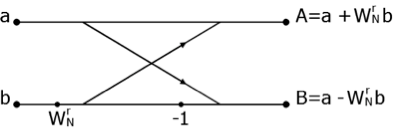
\includegraphics
            [width=0.5\columnwidth]
            {drawings/fftButterfly.png}
	}	
	\caption{Butterfly diagram.}
	\label{fig:FFTButterfly}
\end{figure}

A graphical example of the Cooley-Tukey algorithm applied to an
8-point signal $x$ is shown in figure~\ref{fig:FFT8pts}. The recursion
levels map to stages. In this example, there are $log_2(8)=3$
stages. Each stage has distinctive groups of butterflies called
blocks. The first stage has 4 blocks of a single butterfly, the second
stage has 2 blocks of 2 butterflies and the third stage has a single
block of 4 butterflies.

\begin{figure}[!htb]
	\centering{
      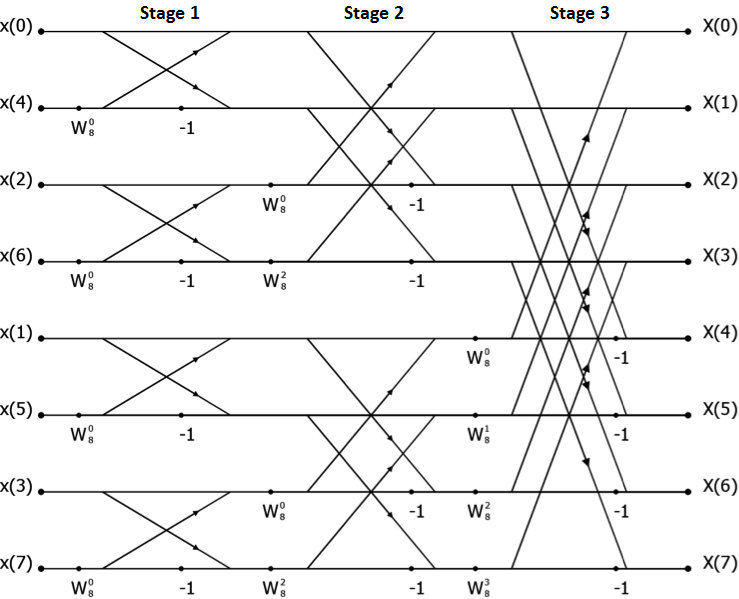
\includegraphics
            [width=0.8\columnwidth]
            {drawings/fft8pts.png}
	}	
	\caption{Cooley-Tukey agorithm appled to an 8-point signal $x$.}
	\label{fig:FFT8pts}
\end{figure}

The Versat FFT kernel implements the Cooley-Tukey algorithm by
splitting a basic butterfly structure in two steps:
\begin{enumerate}
	\item Complex multiplication step: the datapoints stored
          at odd addresses are multiplied by the coefficients
	\item Complex addition step: the datapoints stored at even
          addresses are added and subtracted from the results of the
          first step to yield 2 result datapoints
\end{enumerate}

% ----------------------------------------------------------------------
\subsection{Implementation}
\label{subsection:FFTImplementation}

The FFT kernel follows the algorithm given in the previous subsection,
creating and partially reconfiguring two basic hardware datapaths that
realize the {\em complex multiplication} and {\em complex addition}
steps of the algorithm. In fact, two versions of each datapath have
been created to enable ping-pong data processing. Another datapath is
used to initially reorder the datapoints by reverting the bits of
their addresses. The data format is 32-bit fixed-point in a Q1.31
organization. The kernel is written in the Versat assembly language
and it is 873 instructions long.

The datapath to initially reorder the data is shown in
figure~\ref{fig:mirrorAddresses}. The AGUs of the source memories MEM2
and MEM3 (port A) read the datapoints with the Reverse parameter set
to '1' (table~\ref{tab:MemParameter}), and the AGUs of the destination
memories MEM0 and MEM1 (ports A) write them
sequentially. Concurrently, the table of coefficients is copied from
MEM2 to MEM0 (ports B), so that either can be accessed during the
ping-pong processing.

\begin{figure}[!htb]
\centering
\includegraphics[width=0.8\columnwidth]{drawings/fft-mirrorAddresses.pdf}
\caption{Datapath for read the initial datapoints with mirrored
  addresses.}
\label{fig:mirrorAddresses}
\end{figure}

The Versat controller plays an important role in complex kernels like
the present FFT kernel. It is responsible for generating the
datapaths, reconfiguring them and controlling the algorithm. Namely,
it controls the outer loops over all stages and, in some cases, over
all blocks in a stage.

First, the four datapaths are created and stored in the configuration
memory. They are very similar two by two, swapping only the memories
that are used for reading with the ones that are used for storing the
data. This is done while data is being DMA transferred into the DE.

After reading a number of parameters from the CRF (number of
datapoints, window and overlap sizes and addresses to read/write data
in the external memory), as passed by the host, the program instructs
the DMA to load the first datapoint chunk values in memories MEM2 and
MEM3. Real parts go into MEM2 and imaginary parts into MEM3, not
exceeding the 1024 lower addresses. Coefficient values are also DMA
transferred into memory MEM2, occupying at most the 1024 higher
addresses. Then the data is reordered and placed in memories MEM0 and
MEM1 while the coefficients are copied to MEM0, using the reordering
datapath explained before.

The datapath in figure~\ref{fig:complexMultiplication} implements the
complex multiplication step, reading the data from MEM0 (real part)
and MEM1 (imaginary part) and coefficients from MEM2 (real and
imaginary parts), and writing the result back in MEM0 and MEM1. Its
configuration is loaded from the configuration memory into the
configuration register file in one clock cycle, partially
reconfigured, and shifted to the shadow configuration register in
another cycle. The datapath forms a read-multiply-add-write pipeline
with four multiplications and two additions in parallel in the
respective stages, combining DLP and ILP.

\begin{figure}[!htb]
\centering \includegraphics[width=0.85\columnwidth]{drawings/fft-cmult.pdf}
\caption{Datapath for the complex multiplication step.}
\label{fig:complexMultiplication}
\end{figure}

Next, the datapath that performs the complex addition step, shown in
figure~\ref{fig:complexSum}, is loaded. This datapath performs the two
complex additions in the butterfly diagram of
figure~\ref{fig:FFTButterfly}. Note that MEM0 (real part) and MEM1
(imaginary part) have the original data in the even addresses and the
original data multiplied by the coefficients in the odd
addresses. Therefore the data in the even addresses is added and
subtracted to the data in the odd addresses to produce the two
butterfly outputs. The results are placed in MEM2 (real part) and MEM3
(imaginary part). The parallel additions exploit DLP while the
read-compute-write pipeline exploits ILP.

\begin{figure}[!htb]
\centering \includegraphics[width=0.85\columnwidth]{drawings/fft-csum.pdf}
\caption{Datapath for the complex addition step.}
\label{fig:complexSum}
\end{figure}

After both steps are run, the controller increments the outer loop and
the two steps are applied again, now from MEM2 and MEM3 to MEM0 and
MEM1. This process is repeated until all stages are processed. Every
time the kernel needs more data, the current results are stored in the
external memory and new datapoints are loaded into the DE memories.

Because AGU parameter Period has only 5 bits
(table~\ref{tab:MemParameter}), there is need to break the two step
computations in several parts for some stages. This is because the two
nested loops that can be executed in the DE are used to go over all
blocks and all datapoints within a block. If there are more than
$2^5=32$ butterflies within a block then the inner loop cannot be
used. Only the iterations loop is used and the DE needs to be
reconfigured for each block. In order to save reconfiguration time,
the controller uses partial reconfiguration. Additionally, if an FFT
window cannot fit into the DE memories, the FFT computation is divided
into several smaller FFTs and several other steps to merge the
results.

After all stages are processed, the controller instructs the DMA to
transfer the results to the external memory, using the respective
address in the CRF passed by the host. Then, a new datapoint chunk is
loaded and the whole process starts again, until all datapoints are
processed and stored in the external memory. When this happens, the
algorithm terminates. Before returning to the boot ROM memory, the
controller clears register R0 in the CRF, which signals the host that
Versat has finished execution.

% ----------------------------------------------------------------------
\section{K-Means Clustering}
\label{section:kmeans}

The K-Means algorithm is one of the simplest algorithms for performing
the clustering task. Despite its simplicity, it is still one of the
most widely used clustering algorithms, due to its ease of
implementation and fast execution time.

% ----------------------------------------------------------------------
\subsection{Algorithm}
\label{subsection:kmeansAlgorithm}

The algorithm uses a centroid model. It separates the data into a set
of clusters, each having a centroid represented by the mean vector of
all the datapoints in the cluster. Each datapoint is classified as
being in the cluster whose centroid is closest to it. The Euclidean
distance is a common metric, though other types of metrics can be
applied~\cite{Estlick2001}. For simplicity, the Manhattan Distance
(MD) is used. After an initial position is given to each centroid, the
algorithm starts updating the position of the centers in an iterative
fashion. Each iteration is divided in two main steps:
\begin{enumerate}
	\item Assignment step: each datapoint is assigned to the
          nearest centroid, given the chosen distance metric
	\item Update step: the centroids are recalculated; the new
          positions correspond to the mean of all the datapoints in
          each cluster
\end{enumerate}
The algorithm ends when the centers are unchanged after an iteration.

% ----------------------------------------------------------------------
\subsection{Implementation}
\label{subsection:kmeansImplementation}

The K-Means Clustering kernel follows the algorithm given in the
previous subsection, creating and partially reconfiguring the two
basic hardware datapaths that realize the {\em assignment} and {\em
  update} steps of the algorithm. The kernel is written in the Versat
assembly language and it is 691 instructions long.

As happens in the FFT kernel, the two datapaths are created and stored
in the configuration memory. This is done while the first chunk of
data is being transferred into the DE by the DMA. After reading the
number of points, coordinates, centroids and respective external
memory addresses from the CRF, as passed by the host, the program
instructs the DMA to load the first datapoint chunk and initial
centroid values in memories MEM0 and MEM1, respectively. The datapoint
chunk size cannot exceed 2048x32bits, the size of MEM0 (starting at
the lower address). The number of centroids times the number of
coordinates is limited to 1024x32bits, half the size of MEM1 (starting
at the second half). The other half is reserved for incrementally
building the updated centroids. This is a hard limitation of this
algorithm, which can only be overcome by using a larger embedded
memory for the centroids, which costs silicon, or by streaming the
centroids as done with the datapoints, which penalizes
performance. However, in the target WSN applications, only a few
centroids are used, making the current algorithm implementation
acceptable.

\begin{figure}[!htb]
\centering \includegraphics[width=0.85\textwidth]{drawings/kmeans.pdf}
\caption{Datapath for the assignment step.}
\label{fig:assignment}
\end{figure}

The datapath in figure~\ref{fig:assignment} implements the assignment
step. Its configuration is loaded from the configuration memory into
the configuration register file and shifted to the shadow
configuration register in two clock cycles, as in the FFT kernel. The
DE is started and the first point is compared with all the centroids,
coordinate after coordinate. The absolute value of the coordinate
difference is accumulated in the type II ALU, configured with the {\em
  ACC if A} function. In this function, the A input instructs the ALU
to either store the first absolute difference or accumulate the
following ones. Input A is produced by the AGU from port B of MEM1,
which is thus not used to generate memory addresses -- this is on of
Versat's novel feature as explained in
section~\ref{section:dataEngine}. If $A < 0$ then the ALU stores,
otherwise it accumulates. After processing all coordinates, the MD is
ready. The ALU configured as {\em MIN if A} checks whether the current
centroid is the closest yet to the datapoint, by computing the minimum
between the current MD and the previous minimum. Input A is generated
by port B of MEM2 to synchronize this action. The current MD is
delayed by 1 cycle using the barrel shifter configured as {\em DELAY
  1} (i.e., no shift), so that it can be compared with the current
minimum. If it is smaller, then it will be the next minimum, and the
centroid index, generated by port B of MEM0, is stored in the ALU
configured as {\em REGISTER}, when signalled by port A of MEM2, which
tells when is the new minimum valid. The logic AND between the
existence of a new minimum and the moment when it is valid is
implemented by a multiplier, since all the 6 ALUs have been used
up. Note that port B of MEM0 and both ports of MEM2 need to delay
their start instant considerably, waiting for all coordinates or all
centroids to be processed, plus the datapath latency. This is not
possible to achieve with the 5-bit {\em Delay} AGU parameter given in
table~\ref{tab:MemParameter}, so it is the controller that starts
these AGUs at the right time. Finally, the point label (closest
centroid index) is stored in MEM3 after its port A receives a signal
from the controller at the precise timing after all centroids are
compared to the datapoint.

To process the next datapoint, the DE is partially reconfigured to
advance the addresses of the datapoint and its label in ports A of
MEM0 and MEM3, respectively. It is not possible to advance the
datapoint without reconfiguration, as this would require our AGUs to
support three levels of nested loops when they only support two. Their
2 levels are used to go through all centroids ({\em Iter} = number of
centroids) and all coordinates for each centroid ({\em Per}=number of
coordinates). Also note that we have {\em Shift=-Per} for the AGU of
port A of MEM0, so that its generated address goes back to the first
coordinate after the last one. The partial reconfiguration time for
the next datapoint is hidden, as it occurs while the DE is running the
current datapoint. This process repeats until all datapoints in the
first chunk are processed.

\begin{figure}[!htb]
\centering 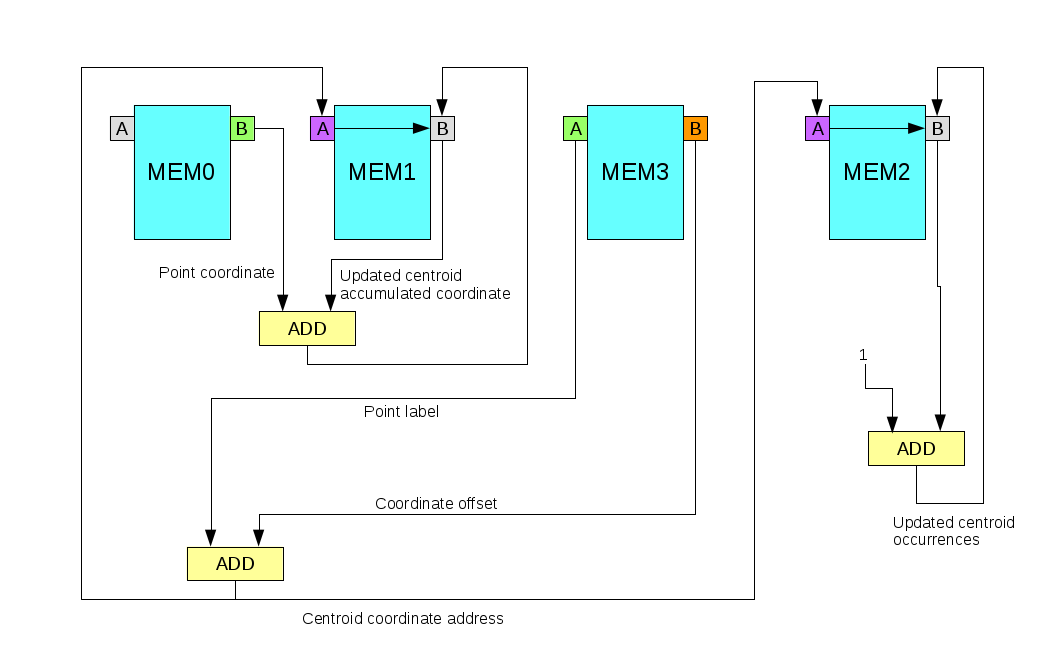
\includegraphics[width=0.85\textwidth]{drawings/kmeans-acc.pdf}
\caption{Datapath for the update step.}
\label{fig:update}
\end{figure}

After the assignment step is done, the datapath for performing the
update step, shown in figure~\ref{fig:update}, is loaded. In this
datapath, the point coordinates, already loaded for the previous step,
are read from port B of MEM0. The point labels (centroid indices),
computed in the previous step, are read from port A of MEM3. Its port
B is generating coordinate offsets synchronized with the datapoint
coordinates. An ALU add labels and coordinate offsets to produce the
accumulated coordinate address of the centroid to update, which is fed
to port A of MEM1. By configuration, port A can serve as the address
for port B, another of Versat's novel features explained in
section~\ref{section:dataEngine}. Thus, the updated centroid
accumulated coordinate is read from port B, added to the current point
coordinate and stored back to port B at the same address. Each port
has an input and an output from which can read an old value and write
a new one to the same address. A similar loop is used for updating the
number of occurrences of each centroid in MEM2, but it only updates
the occurrences once per point. The number of occurrences for each
centroid is stored in MEM2 and is incremented each time it is
addressed, using the same address fed to port A of MEM1. The
incrementer is implemented by another ALU. Note that any FU can select
as input the commonly used constants 0 and 1, instead of a data bus
entry. The two memory read-add-write self loops take 4 clock cycles
due to the accumulated latencies of these operations. Therefore, the
inner loop of the AGUs has size 4 ($Per=4$), and the outer loop size
equals the number of coordinates ($Iter=$ number of coordinates). Also
note that port B of MEM1 and MEM2 are only enabled for writing in the
last cycle of the 4-cycle inner loop ($Duty=1$). After this nested
loop runs, the DE is partially reconfigured to point to the next
datapoint, as is done in the assignment step datapath. This process
repeats until all datapoints in the first chunk are processed.

After the assignment and update steps are run, the next chunk of
datapoints is loaded in MEM0 and the two steps are applied to the new
chunk. This process is repeated until all datapoints are processed.

After all datapoint chunks are processed, the updated centroid
accumulated coordinates reside in MEM1 and must be divided by the
number of occurrences in MEM2 to yield the new centroid
coordinates. Since the DE has no divider, the one that is coupled to
Versat's controller is used to perform the divisions. While the
divider is running, there is time to check whether the newly computed
centroid coordinate differs from the one stored in MEM1, overwriting
it if it does. If none of the new centroids is different from the
stored ones, the algorithm terminates and the final centroids are
DMA transferred to the external memory. If the point labels are also
needed as a final result, then the assignment step must be run again
for all datapoints, as the labels for each data chunk are not
kept. This final loop represents a small overhead if the algorithm has
many iterations. The labels produced during this extra iteration are
DMA transferred to the external memory for each datapoint chunk.

Finally, the program clears register R0 in the CRF, which signals the
host that Versat has finished execution.
